% !TeX root = ../tesis.tex

Let $\vb{E}^\text{i}$ be the electric field of an incident monochromatic plane wave \index{Wave!Plane!Monochromatic} traveling through a non-dispersive medium with refractive index $n_\text{m}$, denominated matrix, in the direction $\vb{k}^\text{i} = k_\text{m}\vu{k}^\text{i}$, with $k_\text{m}$ the wave number of the plane wave into the matrix, and $\vb{E}^\text{sca}$ the electric far field of the scattered field due to a particle with arbitrary shape embedded into the matrix. In general, the scattered electric field propagates in all directions but for a given point $\vb{r} = r\vu{e}_r$ the traveling direction is defined by the vector $\vb{k}^\text{sca} = k_\text{m}\vu{k}^\text{sca} = k_\text{m}\vu{e}_r$.  Due to the linearity of the Maxwell's equations, in the far field  the incident and scattered electric fields are related by a linear relation, that is, 
%
% ---------------------------------- eq: ScatAmpMat ----------------------------------
\begin{equation}
	\vb{E}^\text{sca} = \frac{\exp(\vb{k}^\text{sca}\cdot\vb{r})}{r} \mathbb{F}(\vu{k}^\text{sca}, \vu{k}^\text{i}) \vb{E}^\text{i},
	\label{eq:ScatAmpMat}
\end{equation}
% ---------------------------------- eq: ScatAmpMat ----------------------------------
%
where $\mathbb{F}(\vu{k}^\text{sca}, \vu{k}^\text{i})$ is the scattering  amplitude matrix from direction $\vu{k}^\text{i}$ into $\vu{k}^\text{sca}$ \cite{tsang_scattering_2000}\index{Scattering!Amplitude Matrix}. Since only the far field is considered, both the incident and the scattered electric field can be decomposed into two linearly independent components perpendicular to $\vb{k}^\text{i}$ and $\vb{k}^\text{sca}$, respectively, each forming a right-hand orthonormal system. If the particle acting as a scatterer has a symmetric shape, it is convenient to define the orthonormal systems relative to the scattering plane\index{Plane!Scattering}, which is the plane containing $\vb{k}^\text{i}$ and $\vb{k}^\text{sca}$, since the elements of $\mathbb{F}(\vu{k}^\text{sca}, \vu{k}^\text{i})$ simplify when represented in these bases \cite{tsang_scattering_2000}. By defining the directions perpendicular  ($\perp$) and parallel ($\parallel$) to the scattering plane, the incident and scattered electric fields can be written as
%
% ---------------------------------- eq:Ei // eq:Es ------------------------------ 
\begin{align}
	\vb{E}^\text{i} & = \qty(E_\parallel^\text{i}\vu{e}^\text{i}_\parallel + E_\perp^\text{i} \vu{e}_\perp^\text{i}) \exp(i\vb{k}^\text{i}\cdot\vb{r}),
	\label{eq:Ei} \\
	\vb{E}^\text{sca} & = \qty(E_\parallel^\text{sca}\vu{e}^\text{sca}_\parallel + E_\perp^\text{sca} \vu{e}_\perp^\text{sca}) \frac{\exp(i\vb{k}^\text{sca}\cdot\vb{r})}{r},
	\label{eq:Es}
\end{align}
% ---------------------------------- eq:Ei // eq:Es ------------------------------ 
%
where the harmonic time dependence  $\exp(-i\omega t)$ has been suppressed, and where it has been assumed that the scattered field is described by a spherical wave; the superindex ``$\text{i}$'' (``$\text{sca}$'') denotes the orthonormal system defined by the incident plane wave (scattered fields).  Since $\{\vu{e}_\perp^\text{i}, \vu{e}_\parallel^\text{i},\vu{k}^\text{i} \}$ and $\{\vu{e}_\perp^\text{sca}, \vu{e}_\parallel^\text{sca},\vu{k}^\text{sca} \}$ are right-hand orthonormal systems, they are related by 
%
% ---------------------------------- eq:eParaPerpPerp ------------------------------ 
\begin{align}
	\vu{e}_\perp^\text{i} = \vu{e}_\perp^\text{sca}  & =  \vu{k}^\text{sca} \times \vu{k}^\text{i}, 
	\qquad\qquad
	\vu{e}^\text{i}_\parallel = \vu{k}^\text{i}\times \vu{e}^\text{i}_\perp,
	\qquad\qquad
\vu{e}^\text{sca}_\parallel = \vu{k}^\text{sca} \times \vu{e}_\perp^\text{sca}.
	\label{eq:eParaPerp}
\end{align}
% ---------------------------------- eq:eParaPerpPerp ------------------------------ 
%

As the Eqs. \eqref{eq:eParaPerp} suggest, the unit vector bases of the orthonormal systems relative to the scattering plane depend on the scattering direction. For example, if the incident plane wave travels along the $z$ axis, then $\vu{k}^\text{i} = \vu{e}_z$ and $\vu{k}^\text{sca} = \vu{e}_r$. Thus, according to Eqs. \eqref{eq:eParaPerp}, the unit vector bases of the systems relative to the scatterig plane are   $\vu{e}_\parallel^\text{i} = \cos\varphi \vu{e}_x +\sin\varphi \vu{e}_y$, $\vu{e}_\parallel^\text{sca} = \vu{e}_\theta$ and $\vu{e}_\perp^\text{i} = \vu{e}_\perp^\text{sca}  = - \vu{e}_\varphi$. In Fig. \ref{fig:ScatPlane} the unit vector systems (purple) based on the  scattering plane  (green) defined by the vectors $\vu{k}^\text{i}=\vu{e}_z$ and $\vu{k}^\text{sca} = \vu{e}_r$ are shown, along with the Cartesian (blue) and spherical (black) unit vector bases.
 

\begin{figure}[h!]\centering
	\tdplotsetmaincoords{60}{110}
	\pgfmathsetmacro{\rvec}{1. 3}
	\pgfmathsetmacro{\thetavec}{30}
	\pgfmathsetmacro{\varphivec}{60}
\begin{tikzpicture}[scale=3.5,tdplot_main_coords]
%draw the NP
%	\draw[tdplot_screen_coords,ball color=yellow, opacity = 1] (0,0,0) circle (.05);
%	\draw[tdplot_screen_coords, color=yellow, opacity = 1] (0,0,0) circle (.05);

\pgfmathsetseed{3}
\draw[tdplot_screen_coords, ball color=yellow, opacity = 1,scale =.075]
	 plot [smooth cycle, samples=8,domain={1:8}]
     (\x*360/8+5*rnd:0.5cm+1cm*rnd) node at (0,0) {};
\pgfmathsetseed{3}    
\draw[tdplot_screen_coords, color=yellow, opacity = 1,scale =.075]
	 plot [smooth cycle, samples=8,domain={1:8}]
     (\x*360/8+5*rnd:0.5cm+1cm*rnd) node at (0,0) {};


%set up some coordinates 
	\coordinate (O) at (0,0,0);

%determine a coordinate (P) using (r,\theta,\varphi) coordinates.   This command
%also determines (Pxy), (Pxz), and (Pyz): the xy-, xz-, and yz-projections
%of the point (P). 
%syntax: \tdplotsetcoord{Coordinate name without parentheses}{r}{\theta}{\varphi}
	\tdplotsetcoord{P}{\rvec}{\thetavec}{\varphivec}

%draw figure contents
%--------------------
%draw the main coordinate system axes
	\draw[thick,- latex] (0,0,0) -- (1. 5,0,0) node[anchor=north east]{$x$};
	\draw[thick,- latex] (0,0,0) -- (0,1. 5,0) node[anchor=north west]{$y$};
	\draw[thick,- latex] (0,0,0) -- (0,0,1. 5) node[anchor=south]{$z$};

%draw the main cartesian vector system 
	\draw[thick,- latex, blue] (0,0,0) -- (1,0,0) node[anchor= south east]{$\vu{e}_x$};
	\draw[thick,- latex, blue] (0,0,0) -- (0,1,0) node[anchor=north west]{$\vu{e}_y$};
	\draw[thick,- latex, blue] (0,0,0) -- (0,0,1) node[anchor= east]{$\vu{e}_z$};

%draw a vector from origin to point (P) 
	\draw[thick,color=green, - latex] (O) -- (P);
	\node at (1,. 5,1. 1) {\color{green} $\vb{r}$};

%draw projection on xy plane, and a connecting line
	\draw[dashed, color=green] (O) -- (Pxy);
	\draw[dashed, color=green] (P) -- (Pxy);
	\fill[green, opacity = .3] (O) --(Pxy)-- (P)--(O);
	\draw[- latex, tdplot_screen_coords,green](.42,.2)--(.8,.2);
	\node[tdplot_screen_coords] at (1.2,.2) {\color{green}\small Scattering plane};


%draw the angle \varphi, and label it
	%syntax: \tdplotdrawarc[coordinate frame, draw options]{center point}{r}{angle}{label options}{label}
	\tdplotdrawarc[- latex]{(O)}{0. 5}{0}{\varphivec}{anchor=south}{$\varphi$}


%set the rotated coordinate system so the x'-y' plane lies within the
	%"theta plane" of the main coordinate system
	%syntax: \tdplotsetthetaplanecoords{\varphi}
	\tdplotsetthetaplanecoords{\varphivec}

%draw theta arc and label, using rotated coordinate system
	\tdplotdrawarc[tdplot_rotated_coords, - latex]{(0,0,0)}{0. 45}{0}{\thetavec}{anchor=north}{$\theta$}

%draw some dashed arcs, demonstrating direct arc drawing
	\draw[dashed,tdplot_rotated_coords] (\rvec,0,0) arc (0:90:\rvec);
	\draw[dashed] (\rvec,0,0) arc (0:90:\rvec);

%set the rotated coordinate definition within display using a translation
%coordinate and Euler angles in the "z(\alpha)y(\beta)z(\gamma)" euler rotation convention
%syntax: \tdplotsetrotatedcoords{\alpha}{\beta}{\gamma}
	\tdplotsetrotatedcoords{\varphivec}{\thetavec}{0}

%translate the rotated coordinate system
%syntax: \tdplotsetrotatedcoordsorigin{point}
	\tdplotsetrotatedcoordsorigin{(P)}

%use the tdplot_rotated_coords style to work in the rotated, translated coordinate frame
	\draw[thick,tdplot_rotated_coords,- latex, purple] (0,0,0) -- (. 3,0,0) node[anchor=north west]{{\color{black}$\vu{e}_\theta,$}$\vu{e}_{\parallel}^\text{sca}$};
	\draw[thick,tdplot_rotated_coords,- latex,black] (0,0,0) -- (0,. 3,0) node[anchor=west]{$\vu{e}_\varphi$};
	\draw[thick,tdplot_rotated_coords,- latex,purple] (0,0,0) -- (0,-. 3,0) node[anchor= north west]{$\vu{e}_{\perp}^\text{sca}$};
	\draw[thick,tdplot_rotated_coords,- latex] (0,0,0) -- (0,0,. 3) node[anchor=south]{$\vu{k}^\text{sca}, \vu{e}_r$ };



%set the rotated coordinate definition within display using a translation
%coordinate and Euler angles in the "z(\alpha)y(\beta)z(\gamma)" euler rotation convention
%syntax: \tdplotsetrotatedcoords{\alpha}{\beta}{\gamma}
	\tdplotsetrotatedcoords{\varphivec}{0}{0}

%translate the rotated coordinate system
%syntax: \tdplotsetrotatedcoordsorigin{point}
	\tdplotsetrotatedcoordsorigin{(Pxy)}

	\draw[thick,tdplot_rotated_coords,- latex, purple] (0,0,0) -- (. 3,0,0) node[anchor= west]{$\vu{e}_{\parallel}^\text{i}$};
	\draw[thick,tdplot_rotated_coords,- latex, blue] (0,0,0) -- (0,0,. 3) node[anchor= west]{$\vu{e}_z$};	
	\draw[thick,tdplot_rotated_coords,- latex, purple] (0,0,0) -- (0,-. 3,0) node[anchor= north west]{$\vu{e}_{\perp}^\text{i}$};



% Plane Wave
	\foreach \i in {-7,...,-2}{
		\draw[thick,tdplot_screen_coords,red, - latex] (\i/10,0,0)--(\i/10,1,0);}
	\node[tdplot_screen_coords] at (-4.5/10,1.1,0){\color{red}$\vb{k}_i$};
	\node[tdplot_screen_coords] at (-4.5/10,-.15,0){\begin{minipage}{2.cm}\centering\small \color{red}Incident plane wave\end{minipage}};
\end{tikzpicture}
%
\caption[Scattering plane unit vector systems]{The scattering plane (green) is defined by the vectors $\vu{k}^\text{i}$, direction of the incident plane wave (red), and $\vu{k}^\text{sca}$, direction of the scattered field in a given point $\vec{r}$. If the direction of the incident plane wave is chose to be $\vu{e}_z$, the parallel and perpendicular components of the incident field relative to the scattering plane are $\vu{e}_\parallel^\text{i} = \cos\varphi\vu{e}_x +\sin\varphi\vu{e}_y$ and  $\vu{e}_\perp^\text{i} = -\vu{e}_\varphi$, while the components of the scattering field relative to the scattering plane are $\vu{e}_\parallel^\text{sca} = \vu{e}_\theta$, $\vu{e}_\perp^\text{sca} = - \vu{e}_\varphi$. The cartesian unit vector basis is shown in blue, the spherical unit vector basis in black, while the basis of the orthonormal systems relative to the scattering plane are shown in purple. }
\label{fig:ScatPlane}
	\end{figure}	

After a incident plane wave interacts with a particle, the total electric field outside the particle is given by the sum of the incident and the scattered fields. Therefore the power per unit  the time averaged Poynting vector, denoting the power flow per unit area, of the total field is given by 
%
% ---------------------------------------------------------
\begin{align}
\ev{\vb{S}}_t 
		= \underbrace{\frac12 \Re \qty(\vb{E}^\text{i}\times\vb{H}^\text{i*})}_{\text{\normalsize $\ev{\vb{S}^\text{i}}_t $}} + 
		\underbrace{\frac12 \Re \qty(\vb{E}^\text{sca}\times\vb{H}^\text{sca*})}_{\text{\normalsize $\ev{\vb{S}^\text{sca}}_t $}}+
		\underbrace{	\frac12 \Re\qty(\vb{E}^\text{i}\times\vb{H}^\text{sca*} + \vb{E}^\text{sca}\times\vb{H}^\text{i*})}_{\text{\normalsize$\ev{\vb{S}^\text{ext}}_t$}},
\label{eq:Stot}
\end{align}
% ---------------------------------------------------------
%
where it is separated into three contributions: the incident field, the scattered field and their cross product denoted by extinction field. By means of the Faraday-Lens Law and Eq. \eqref{eq:ScatAmpMat}, the  contribution to the Poynting vector from the incident and the scattered fields can be rewritten as\index{Poynting vector}
%
% ------------------ Si
\begin{equation}
\ev{\vb{S}^\text{i}}_t = \frac{\norm{\vb{E}^\text{i}}^2}{2 Z_\text{m}}\norm{\vb{E}^\text{i}}^2\vu{k}^\text{i},
\qquad\text{and}\qquad
\ev{\vb{S}^\text{sca}}_t = \frac{\norm{\vb{E}^\text{sca}}^2}{2 Z_\text{m}}\vu{k}^\text{sca} 
						=  \frac{\norm{\mathbb{F}(\vu{k}^\text{sca},\vu{k}^\text{i})\vb{E}^\text{i}}^2}{2 Z_\text{m}r}\vu{k}^\text{sca},
\end{equation}
% ------------------- Si
%
with $Z_\text{m}$ the impedance of the non-dispersive matrix, while the extinction field contribution is given by
%
% ------------------ Si
\begin{align}
\ev{\vb{S}^\text{ext}}_t = &\Re\left\{
									\frac{\exp[-i(\vb{k}^\text{sca}-\vb{k}^\text{i})\cdot\vb{r}]}{2 Z_\text{m}r^2}
									\qty[\vu{k}^\text{sca}\qty(\vb{E}^\text{i}\cdot \mathbb{F}^*\vb{E}^\text{i*})     
										-\qty(\mathbb{F}\vb{E}^\text{i*})	\qty(\vb{E}^\text{i}\cdot\vu{k}^\text{sca})]
								 \right.\notag	\\
								&\hspace{2em}\left.
								+\frac{\exp[i(\vb{k}^\text{sca}-\vb{k}^\text{i})\cdot\vb{r}]}{2 Z_\text{m}r^2}
									\qty[\vu{k}^\text{i}\qty(\vb{E}^\text{i*}\cdot \mathbb{F}\vb{E}^\text{i})     
										-\qty(\vb{E}^\text{i*})	\qty(\mathbb{F}\vb{E}^\text{i}\cdot\vu{k}^\text{i})]	\right\},					
\end{align}
% ------------------- Si
%
where the scattering amplitude matrix is evaluated as $\mathbb{F}(\vu{k}^\text{sca},\vu{k}^\text{i})$.

The power scattered by the particle can be calculated by integrating $\ev{\vb{S}^\text{sca}}_t$ in a closed surface surrounding the particle and by normalizing the power scattered by $\norm{\ev{\vb{S}^\text{i}}_t}$, a quantity with units of area is obtain; this quantity is known as scattering cross section denoted by $C_\text{sca}$ and given by
%
% ------------------ Si
\begin{tcolorbox}[title = Scattering Cross Section,	ams align, breakable]
C_\text{sca} = \int_{4\pi}\frac{\norm{\vb{E}^\text{sca}}^2}{\norm{\vb{E}^\text{i}}^2}\vu{k}^\text{sca}\cdot\vu{e}_r r^2\dd{\Omega} = \int_{4\pi}\frac{\norm{\mathbb{F}(\vu{k}^\text{sca},\vu{k}^\text{i})\vb{E}^\text{i}}^2}{\norm{\vb{E}^\text{i}}^2}\dd{\Omega} .
\label{eq:Csca}
\end{tcolorbox}

% ------------------- Si
%

In a similar manner, an absorption cross section $C_\text{abs}$ can be defined. One way to define it is to consider the Joule's Heating Law \cite{tsang_scattering_2000}\index{Joule!Heating Law} and assuming an Ohmic material for the particle\index{Ohm!Law} with a conductivity $\sigma = i\omega n_p^2$ \cite{jackson_classical_1999} and a refractive index $n_p$, that is,
%
% ------------------ Si
\begin{tcolorbox}[title = Absorption Cross Section,	ams align, breakable]
C_\text{abs} = \frac12\int \frac{\Re(\vb{j}\cdot \vb{E}^\text{int*})}{\norm{\vb{E}^\text{i}}^2/2Z_\text{m}}\dd{V}
			= \int\omega \Re(n_p)\Im(n_p) \frac{\norm{\vb{E}^\text{int}}^2}{\norm{\vb{E}^\text{i}}^2/2Z_\text{m}} \dd{V},
			\label{eq:Cabs}
\end{tcolorbox}
% ------------------- Si
%
where  $\vb{j}$ is the electric currents inside the particle and $\vb{E}^\text{int}$ the total electric field inside of the particle, where the integration is performed. Yet, another method to calculate $C_\text{abs}$ is by performing the closed surface integral of Eq. \eqref{eq:Stot} and normalizing by $\norm{\ev{\vb{S}^\text{i}}_t}$, leading to
%
% -----------------------------
\begin{align}
C_\text{abs} = & - \frac{2Z_\text{m}}{\norm{\vb{E}^\text{i}}^2}\int\qty(\ev{\vb{S}^\text{i}}_t + \ev{\vb{S}^\text{sca}}_t + \ev{\vb{S}^\text{ext}}_t)\cdot\vu{e}_rr^2\dd{\Omega} 
					\notag \\
			=  & - C_\text{sca} - \frac{2Z_\text{m}}{\norm{\vb{E}^\text{i}}^2}\int   \ev{\vb{S}^\text{ext}}_t\cdot \vu{e}_r\dd{\Omega}
\label{eq:CabsScaInt}
\end{align}
% ------------------------------
%
where the contribution of $\ev{\vb{S}^\text{i}}_t$ to the integral is zero since a non-dispersive matrix was assumed. To solve the integral in Eq. \eqref{eq:CabsScaInt} let us define $\theta$ as the angle between $\vu{k}^\text{sca}$ and $\vu{k}^\text{i}$ as the polar angle  and  $\varphi$ as the azimuthal angle as shown in Fig \ref{fig:ScatPlane}. With this election of coordinates, one can define the extinction cross section $C_\text{ext}$ as
%
% -----------------------------
\begin{align}
C_\text{ext} = - &\Re \left\{  
			 \frac{\exp(-ik_mr) }{\norm{\vb{E}^\text{i}}^2}\int \exp(ik_mz\cos\theta)(1)\qty(\vb{E}^\text{i}\cdot \mathbb{F}^*\vb{E}^\text{i*})  \dd{\Omega} \right.	\notag\\
			&\hspace*{2em}\frac{\exp(ik_mr) }{\norm{\vb{E}^\text{i}}^2}\int \exp(-ik_mz\cos\theta)\cos\theta \qty(\vb{E}^\text{i*}\cdot \mathbb{F}\vb{E}^\text{i})     \dd{\Omega} 	\notag\\
			&\hspace*{2em}\left.\frac{\exp(ik_mr) }{\norm{\vb{E}^\text{i}}^2} \int \exp(-ik_mz\cos\theta)(\sin\theta\cos\varphi+\sin\theta\sin\varphi) \qty(\vb{E}^\text{i*}\cdot \mathbb{F}\vb{E}^\text{i})    \dd{\Omega}  \right\},
\label{eq:CextFull}
\end{align}
% ------------------------------
%
where the relations $\vu{k}^\text{sca}\cdot\vu{e}_r = 1$, $\vu{k}^\text{i}\cdot\vu{e}_r = \cos\theta$, $\vu{E}^\text{i}\cdot\vu{e}_r= (\sin\theta\cos\varphi+\sin\theta\sin\varphi)$ and  $\vb{E}^\text{sca}\cdot\vu{e}_r = 0$ were employed. The integrals in Eq. \eqref{eq:CextFull} can be solved by a two fold integration by parts on the variable $\cos\theta$ and by depreciating the terms proportional to $r^{-2}$; this process leads to a zero contribution from the third term of Eq. \eqref{eq:CextFull}. After arranging the results of the two fold integration by parts on the first two terms of Eq. \eqref{eq:CextFull}, one can proof that the extinction cross section depend only in the forward direction $\theta = 0$ as follows \cite{bohren_absorption_1983}
%
% -----------------------------
\begin{tcolorbox}[title = Extinction Cross Section,	ams align, breakable]
		C_\text{ext} = \frac{4\pi}{k_m^2 \norm{\vb{E}^\text{i}}^2}&\Re\qty[ \vb{E}^\text{i}\cdot \mathbb{F}^*(\vu{k}^\text{sca},\vu{k}^\text{i}) \vb{E}^\text{i*} ]\eval_{\theta = 0}.
\label{eq:Cext}
\end{tcolorbox}
% ------------------------------
%
Thus, the absorption cross section can be obtained from Eqs. \eqref{eq:CabsScaInt} and \eqref{eq:Cext}, and this expression is one form of the so called optical theorem \cite{newton_optical_1976,bohren_absorption_1983}.
%
%
\begin{tcolorbox}[title = Optical Theorem,	ams align, breakable]
		C_\text{abs} = C_\text{ext} - C_\text{sca}.
		\label{eq:OptTheorem}
\end{tcolorbox}














%
\begin{figure}[h!]\centering
	\begin{subfigure}{.05\textwidth}\caption{}\label{sfig:secondary1}\vspace*{5.5cm}\end{subfigure}
	\hspace*{-2.em}
	\begin{subfigure}{.48\textwidth} 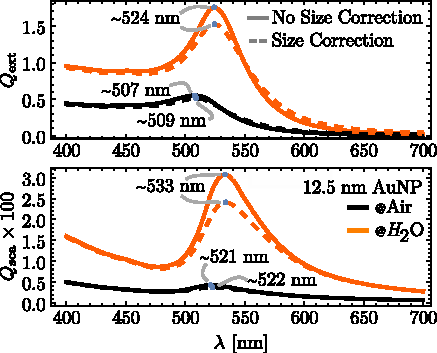
\includegraphics[scale = 1.02]{1-Theory/figs/QextQsca_12-5.pdf}\end{subfigure}
	\hspace*{-.5em}\begin{subfigure}{.05\textwidth}\vspace{-5.5cm}\caption{}\label{sfig:secondaty2}	\end{subfigure}
	\hspace*{-2.em}
	\begin{subfigure}{.48\textwidth} 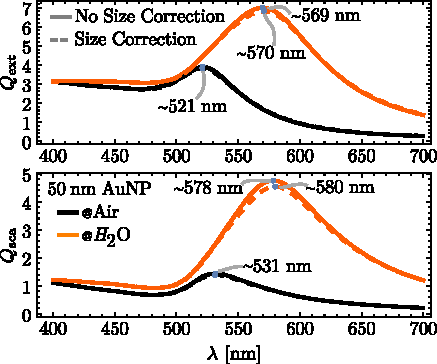
\includegraphics[scale = 1.02]{1-Theory/figs/QextQsca_50.pdf}\end{subfigure}%
\vspace*{-.5em}
\caption[Example of Figure title]{The explanation of your figures. \blindtext}	\label{fig:Main}	
\end{figure}	
				
\begin{figure}[h!]\centering
	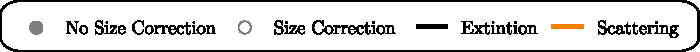
\includegraphics[scale=1]{1-Theory/figs/legend.pdf}\\[.5em]
%
	\hspace*{2em}\begin{subfigure}{.05\textwidth}\caption{}\label{sfig:secondary1}\vspace*{6.35cm}\end{subfigure}
	\hspace*{-3.50em}
	\begin{subfigure}{.24\textwidth} 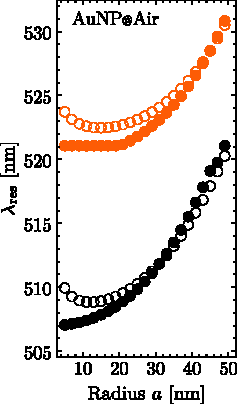
\includegraphics[scale = 1]{1-Theory/figs/redShift_rad1.pdf}\end{subfigure}
%	
	\hspace*{.25em}\begin{subfigure}{.05\textwidth}\vspace{-6.35cm}\caption{}\label{sfig:secondaty2}	\end{subfigure}
	\hspace*{-2.5em}
	\begin{subfigure}{.24\textwidth} 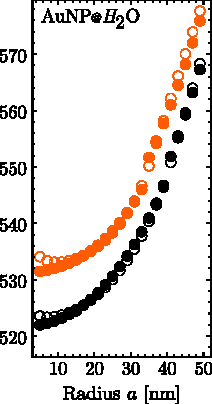
\includegraphics[scale = 1]{1-Theory/figs/redShift_rad2.pdf}\end{subfigure}%
%
	\hspace*{-.5em}\begin{subfigure}{.05\textwidth}\vspace{-6.35cm}\caption{}\label{sfig:secondaty2}	\end{subfigure}
	\hspace*{-2.45em}
	\begin{subfigure}{.24\textwidth} 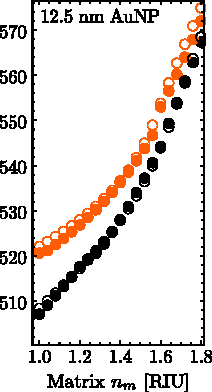
\includegraphics[scale = 1.02]{1-Theory/figs/redShift_mat1.pdf}\end{subfigure}%
%
	\hspace*{-.45em}\begin{subfigure}{.05\textwidth}\vspace{-6.35cm}\caption{}\label{sfig:secondaty2}	\end{subfigure}
	\hspace*{-2.45em}
	\begin{subfigure}{.24\textwidth} 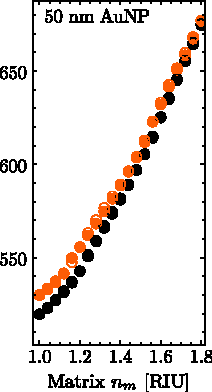
\includegraphics[scale = 1.02]{1-Theory/figs/redShift_mat2.pdf}\end{subfigure}%	
\vspace*{-.5em}
\caption[Example of Figure title]{The explanation of your figures. \blindtext}
\label{fig:Main}	
\end{figure}	







































